\begin{figure}[H]
  \centering
    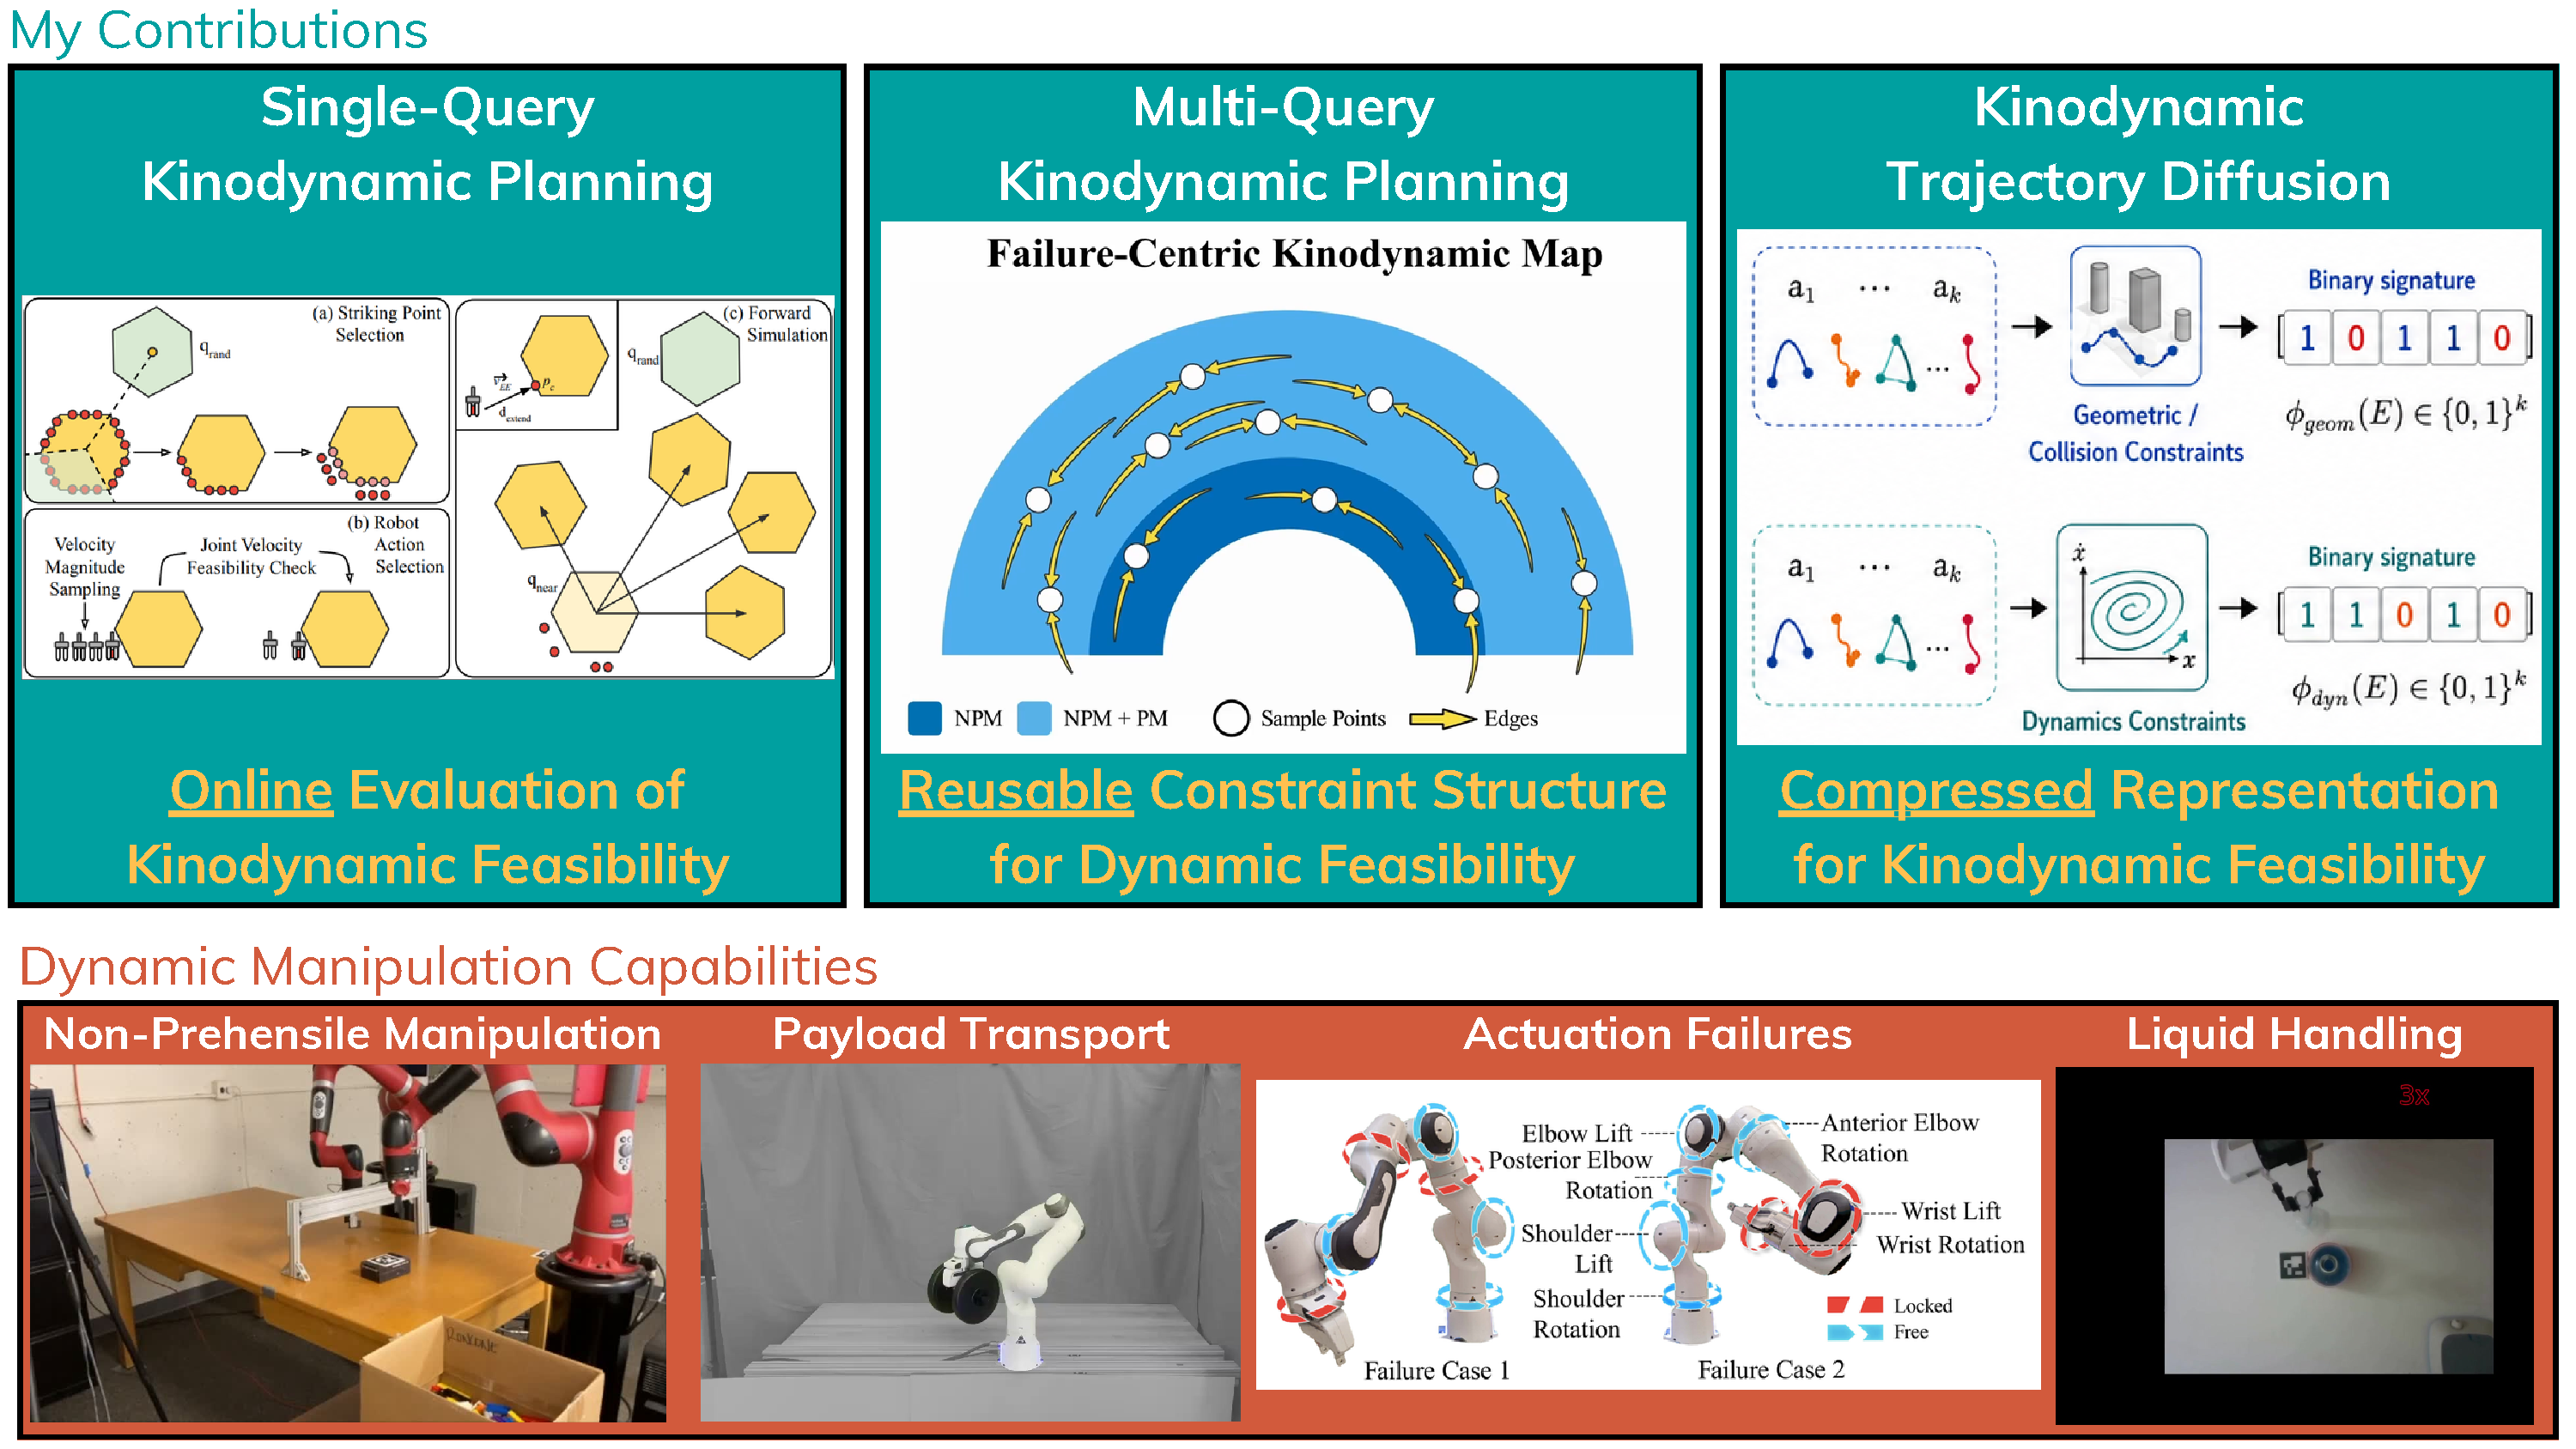
\includegraphics[width=\textwidth]{figs/outline.pdf}
  \caption[Overview of thesis work from kinodynamic planning to diffusion-based generation.]{My thesis work progresses from sampling-based kinodynamic planning to diffusion-based trajectory generation, leveraging various modeling approaches applied to a broad class of manipulation problems that are subject to both kinematic and dynamic constraints.}\label{fig:outline}
\end{figure}
\section{Contributions}


\subsection{Thesis and Approach}
\label{sec:intro:statement}

This dissertation develops planning and learning methods for dynamic manipulation that expand robot capability beyond predominantly geometric pick-and-place to tasks governed by contact dynamics, object inertia, and physical parameter variation.
Three families of methods are developed, each incorporating dynamic feasibility into the motion generation process differently:

\paragraph{Part I: Online Constraint Evaluation.}
The first part develops dynamics-aware planning methods for non-prehensile manipulation involving impulsive contact, coupled robot-object dynamics, and liquid transport, exploiting physical constraints directly through kinodynamic primitives and simulation-based forward reasoning.
In this setting, the planner maintains an explicit connection between sampled actions and dynamically feasible outcomes, but pays the cost of physics-based reasoning during each planning query.
\begin{enumerate}
  % \item \textbf{A design framework for dynamics-aware motion generation} (\cref{ch:prior}).
        % A conceptual framework organizing manipulation methods along four design axes---modeling burden, problem dimensionality, system integration, and usability---providing a unified perspective on the tradeoffs underlying dynamics-aware planning systems.

  \item \textbf{PokeRRT: impulsive non-prehensile manipulation through kinodynamic search} (\cref{ch:poking}).
        A sampling-based kinodynamic planner that uses physics simulation as a forward model for object rearrangement via impulsive contact, without requiring explicit contact models.
        Across six scenarios, poking achieves higher success rates and lower task completion times than pushing and grasping baselines.

  \item \textbf{Kinodynamic planning under coupled robot-object dynamics} (\cref{ch:constrained}).
        Extensions of kinodynamic planning to manipulation tasks governed by coupled dynamics, including whole-body manipulation under locked multi-joint failures and spill-free liquid transport in cluttered environments.
        These methods maintain up to 92\% of nominal reachable workspace under failures and expand feasible spill-free solution spaces by up to $3\times$ over prior approaches.
\end{enumerate}

\paragraph{Part II: Amortized Feasibility via Reusable Motion Structure.}
The second part develops lazy reusable kinodynamic planning representations for multi-query manipulation, reducing repeated planning cost while preserving explicit dynamically feasible motion structure across related problems.
Physical admissibility is not fully relearned or recomputed from scratch; instead, prior feasibility computation is stored in a reusable structure and selectively validated when needed.
\begin{enumerate}
  \setcounter{enumi}{2}
  \item \textbf{LazyBoE: multi-query kinodynamic planning via lazy edge bundles} (\cref{ch:multiquery}).
        A multi-query kinodynamic planner that amortizes dynamics computation across repeated planning problems by precomputing control-parameterized edge bundles over discretized state and control spaces.
        Lazy propagation and collision checking substantially reduce repeated planning cost while preserving kinodynamic feasibility.
\end{enumerate}

\paragraph{Part III: Amortized Feasibility via Learned Generative Models.}
The third part develops conditional generative models for dynamic manipulation that rapidly sample trajectories conditioned on physical parameters such as payload mass and embodiment configuration.
The thesis further considers the problem of constraint identification, reframing it in terms of induced behavior rather than perceptual or parameter similarity.
In these cases, targeted constraint probes are used to construct compact behavioral signatures that expose hidden differences between environments with similar appearance but different admissible behaviors.
\begin{enumerate}
  \setcounter{enumi}{3}
  \item \textbf{Motion generation as conditional sampling} (\cref{ch:generation}).
        A reformulation of dynamics-aware motion generation as conditional trajectory sampling, establishing a conceptual bridge between kinodynamic planning and learned generative models.

  \item \textbf{Conditional trajectory diffusion for dynamic constraint satisfaction} (\cref{ch:payload}).
        A diffusion-based trajectory generator conditioned on task-level dynamic properties such as payload mass and embodiment configuration.
        The method achieves super-nominal payload manipulation---67.6\% workspace accessibility at $3\times$ rated payload capacity---in approximately 10\,ms without runtime constraint checking, and generalizes to fail-active manipulation under actuation failures.

  \item \textbf{Task-agnostic trajectory seeding for constrained optimization} (\cref{ch:seeding}).
        A conditioning mechanism that represents kinematic and dynamic constraints as robot state samples in order to generate near-feasible trajectory seeds for constrained optimization.
        The approach improves solver convergence and feasibility across diverse manipulation tasks without task-specific engineering.
\end{enumerate}

% Across all three parts, the goal remains the same: enabling robots to reason about and exploit dynamic constraints rather than deferring to geometric abstractions---and making the representation of that knowledge an explicit design decision.

% \subsection{Contributions}
% \label{sec:intro:contributions}

% This thesis develops methods for dynamic manipulation planning and learning, organized into three groups by approach.

% \paragraph{Online Constraint Evaluation: Kinodynamic Planning.}

% \paragraph{Amortized Feasibility via Reusable Motion Structure.}

% \paragraph{Amortized Feasibility via Learned Generative Models.}
